\documentclass[11pt, a4paper]{article}

\usepackage[utf8]{inputenc}
\usepackage[T1]{fontenc}
\usepackage{amsmath}
\usepackage{amssymb}
\usepackage{graphicx}
\usepackage{geometry}
\usepackage{fancyhdr}
\usepackage{enumitem}
\usepackage{array}
\usepackage{eso-pic}

\usepackage{siunitx}
\DeclareSIUnit{\litre}{l}
\sisetup{angle-symbol-degree = ^\circ}
\sisetup{locale = DE, separate-uncertainty, inter-unit-product = {},
range-units = brackets, list-units = single, per-mode=symbol-or-fraction}

\makeatletter
\def\input@path{{./}{../../}}
\makeatother
\graphicspath{{./}{../../}}

\geometry{a4paper, top=2.5cm, bottom=2.5cm, left=2.5cm, right=2.5cm}

\input{defs}

\pagestyle{fancy}
\fancyhf{}
\cfoot{\thepage}

\begin{document}
\AddToShipoutPictureBG*{%
  \AtPageUpperLeft{%
    \hspace{2.0cm}%
    \raisebox{-5.cm}{%
      
\includegraphics[width=4cm]{Bilder/Allgemein/LogoFHCampus.png}%
    }%
  }%
}

\begin{center}
    {\Large \textbf{Physikalische Grundlagen}} \\[1em]
    {\large 1. Schriftliche Prüfung: Sommersemester 2026} \\[1em]
    {\large Studiengang: Clinical Engineering}
\end{center}

\vspace{1cm}

\noindent
\begin{tabular}{ll}
    \textbf{Vorname:} & \underline{\hspace{8cm}} \\[0.3cm]
    \textbf{Nachname:} & \underline{\hspace{8cm}} \\
\end{tabular}

\vspace{1cm}

\begin{itemize}[label={$\Diamond$}]
    \item Sie haben 90 min Zeit.
    \item Es sind keine Unterlagen erlaubt.
    \item Sie dürfen einen Taschenrechner verwenden.
    \item Geben Sie klare und verständliche Antworten.
    \item Schreiben Sie leserlich.
    \item Streichen Sie alle bis auf eine Lösung durch.
    \item Jeglicher Versuch unerlaubte Hilfsmittel zu verwenden oder von KommilitonInnen \\
    abzuschreiben, wird mit einer negativen Bewertung des Tests geahndet.
\end{itemize}

\vspace{1cm}

\begin{center}
    \textbf{Viel Erfolg!}
\end{center}

\vspace{2cm}

\begin{flushright}
    \renewcommand{\arraystretch}{1.23}
    \begin{tabular}{l p{2.3cm}}
        \hline
        \noalign{\vskip 0.15cm}
        \textbf{\Large{Punkte:}} & \textbf{\Large{/49}} \\
        \noalign{\vskip 0.1cm}
        \hline
        Beispiel 1: & /12 \\
        Beispiel 2: & /14 \\
        Beispiel 3: & /13 \\
        Beispiel 4: & /10
    \end{tabular}
\end{flushright}

\newpage

\section*{Beispiel 1 - Mischtemperatur}

\begin{minipage}[t]{0.62\textwidth}
    \vspace{0pt}
    Ein \SI{600}{\gram} schweres Stück Kupfer mit einer Temperatur von $T_{\text{Cu}} = \SI{180}{\degreeCelsius}$ wird in ein wärmeisoliertes Gefäß mit \SI{1.5}{\litre} Wasser gegeben. Das Wasser hat anfangs eine Temperatur von $T_{\text{W}} = \SI{22}{\degreeCelsius}$.

    Gegeben sind die spezifische Wärmekapazität von Kupfer $c_{\text{Cu}} = \SI{0.385}{\kilo\joule\per(\kilogram\cdot\kelvin)}$, die spezifische Wärmekapazität von Wasser $c_{\text{W}} = \SI{4.18}{\kilo\joule\per(\kilogram\cdot\kelvin)}$ und die Dichte von Wasser $\rho_{\text{W}} = \SI{1.0}{\kilogram\per\deci\metre\cubed}$.
\end{minipage}\hfill
\begin{minipage}[t]{0.33\textwidth}
    \vspace{0pt}
    \centering
    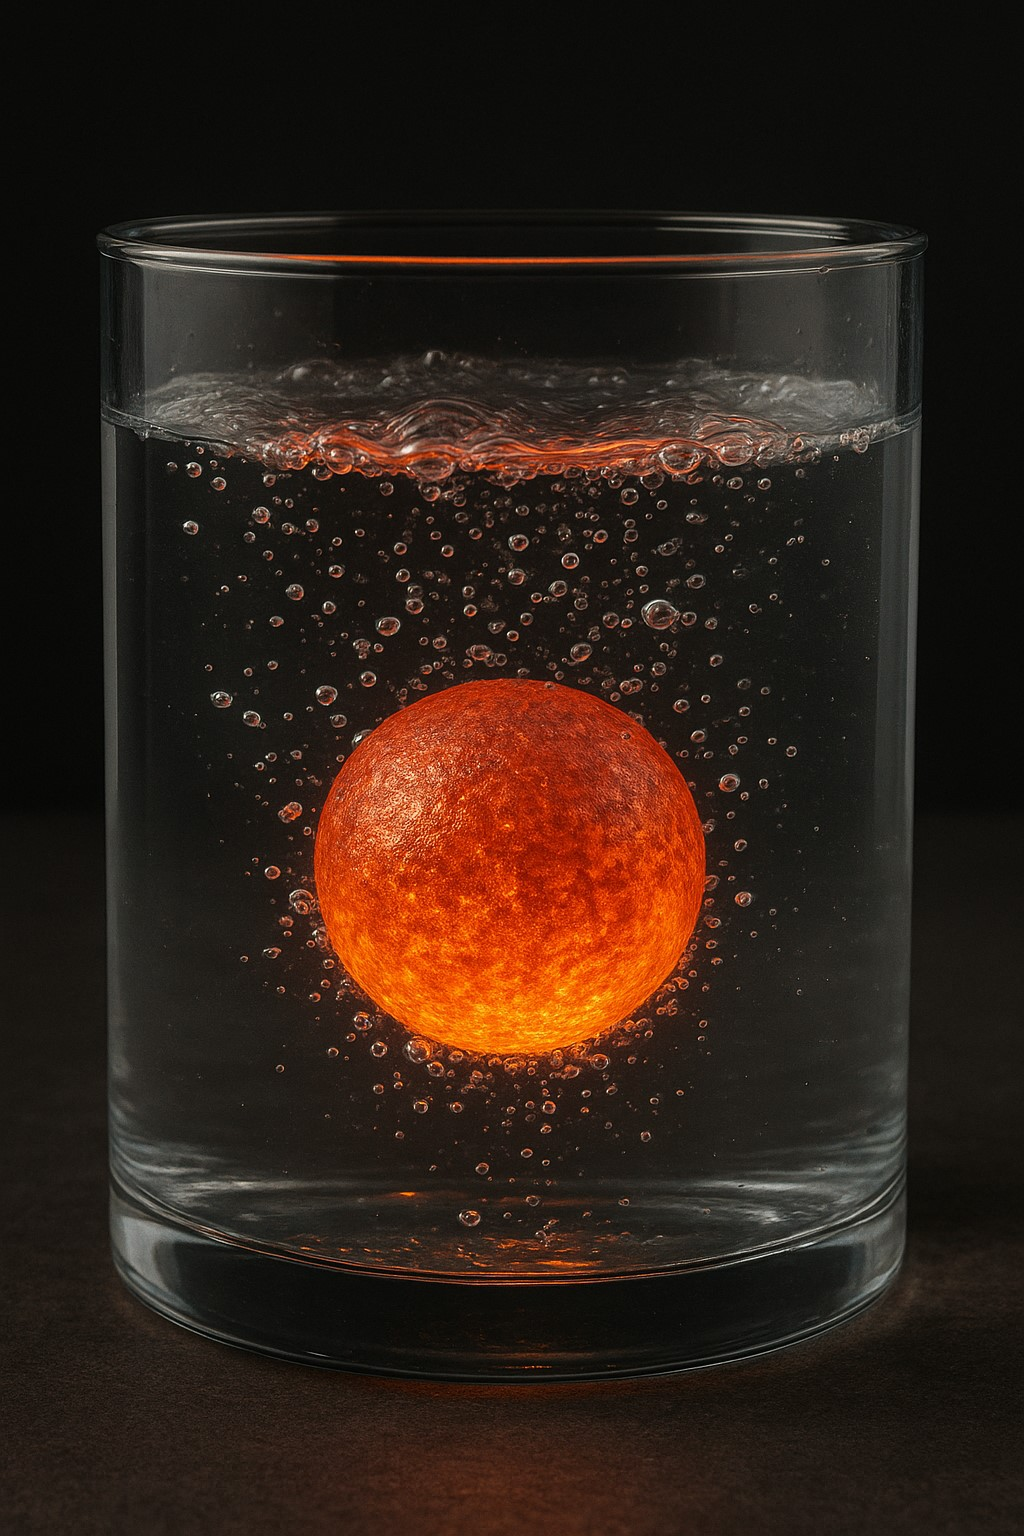
\includegraphics[width=0.8\textwidth]{Bilder/Test/3terAntritt/kugel_in_wasser_3.jpeg}
\end{minipage}

\subsection*{Aufgabe}
Berechnen Sie die Endtemperatur $T_{\text{Misch}}$, die sich im thermischen Gleichgewicht einstellt. Nehmen Sie an, dass keine Wärme an die Umgebung verloren geht.

\subsection*{Vorgehen}
\begin{enumerate}
    \item Formulieren Sie den Grundsatz des thermischen Gleichgewichts für dieses isolierte System.
    \item Berechnen Sie die Masse des Wassers.
    \item Stellen Sie die Formel für die vom Kupfer abgegebene Wärme $Q_{\text{ab}}$ als Funktion von $T_{\text{Misch}}$ auf.
    \item Stellen Sie die Formel für die vom Wasser aufgenommene Wärme $Q_{\text{auf}}$ als Funktion von $T_{\text{Misch}}$ auf.
    \item Setzen Sie die beiden Wärmeformeln gleich und berechnen Sie die Mischtemperatur.
\end{enumerate}

\vfill
\begin{flushright}
\renewcommand{\arraystretch}{1.23}
\begin{tabular}{|c | c | c | c | c|}
\hline
\multicolumn{5}{|l|}{\textbf{\large{Punkte: \quad\quad\quad /12}}}\\
\hline
\textbf{1)} & \textbf{2)} & \textbf{3)} & \textbf{4)} & \textbf{5)} \\
\quad/1 & \quad/2 & \quad/2 & \quad/2 & \quad/5 \\
\hline
\end{tabular}
\end{flushright}

\newpage

\section*{Beispiel 2 - Rutsche mit Reibung}

\begin{minipage}[t]{0.5\textwidth}
    \vspace{0pt}
    Ein Kind mit einer Masse von $m = \SI{35}{\kilogram}$ startet aus dem Stillstand am oberen Ende einer geraden Rutsche. Die Rutsche hat eine Höhe von $h = \SI{3}{\metre}$ und eine Länge von $L = \SI{5}{\metre}$. Der Gleitreibungskoeffizient zwischen Kind und Rutsche beträgt $\mu_{\text{Gleit}} = \num{0.20}$. Die Erdbeschleunigung ist $g = \SI{9.81}{\metre\per\second\squared}$.
\end{minipage}\hfill
\begin{minipage}[t]{0.47\textwidth}
    \vspace{0pt}
    \centering
    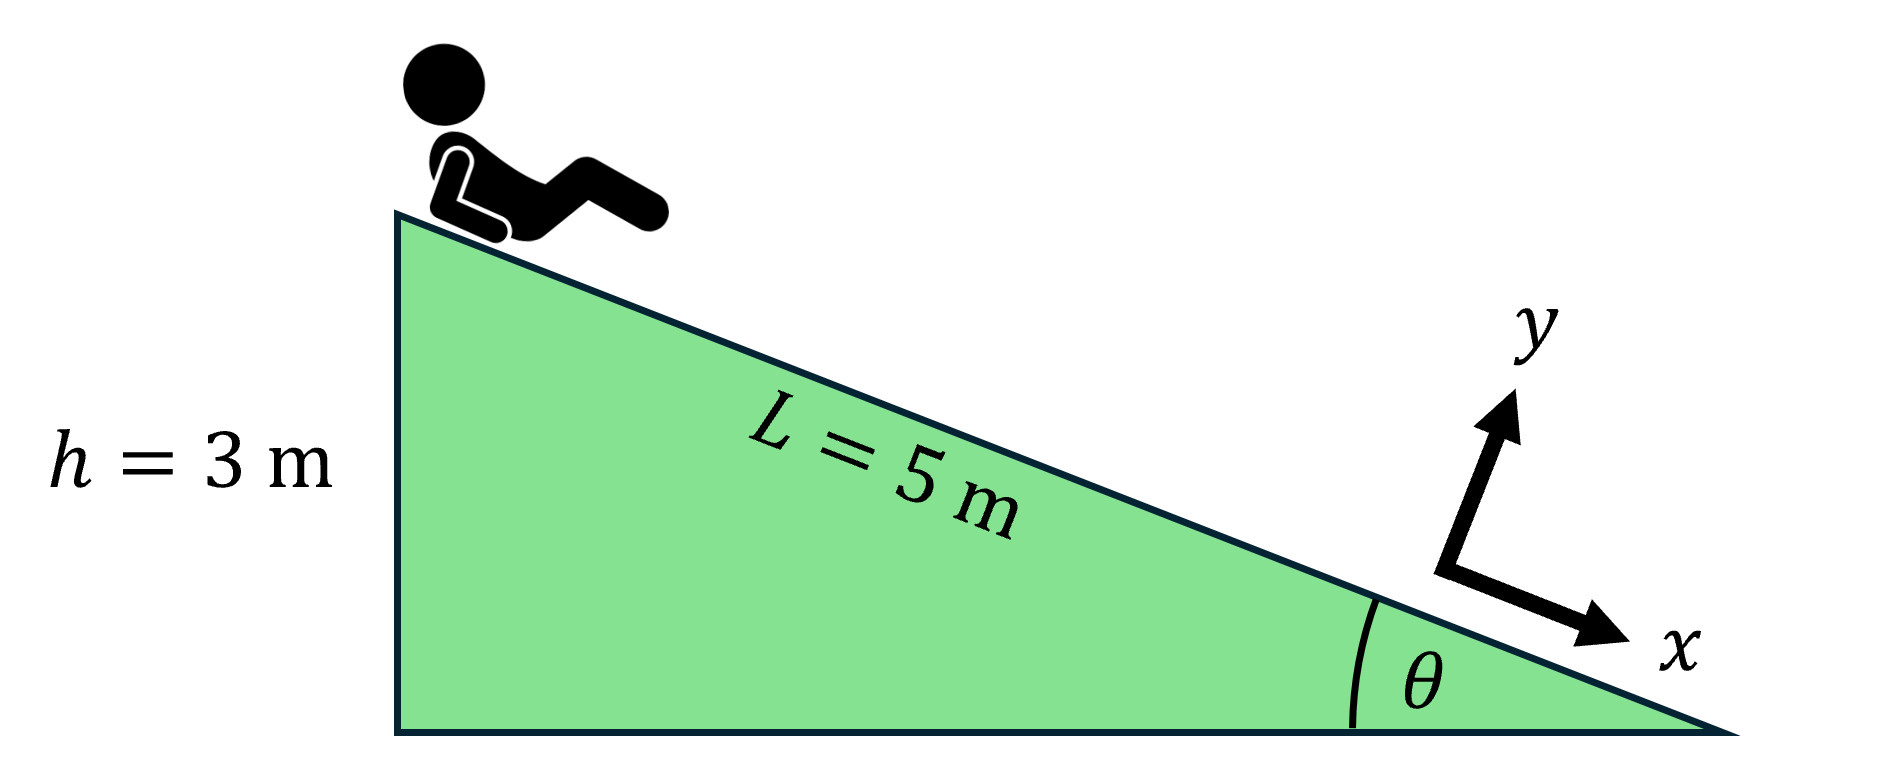
\includegraphics[width=0.98\textwidth]{Bilder/Uebungsaufgaben/kind_rutsche.png}
\end{minipage}

\subsection*{Aufgabe}
Berechnen Sie die Endgeschwindigkeit des Kindes am unteren Ende der Rutsche.

\subsection*{Vorgehen}
\begin{enumerate}
    \item Zeichnen Sie alle auf das Kind wirkenden Kräfte in die Skizze ein: Gewichtskraft, Normalkraft und Gleitreibungskraft.
    \item Berechnen Sie den Neigungswinkel $\theta$ der Rutsche.
    \item Zerlegen Sie die Gewichtskraft in eine Komponente senkrecht ($F_{G, \perp}$) und eine parallel ($F_{G, \parallel}$) zur Rutschfläche. Geben Sie die Formeln und Zahlenwerte an.
    \item Berechnen Sie die Normalkraft $F_N$ und daraus die Gleitreibungskraft $F_{R, \text{Gleit}}$.
    \item Berechnen Sie die resultierende Nettokraft in Bewegungsrichtung (Hangabtrieskraft) und daraus die konstante Beschleunigung des Kindes entlang der Rutsche.
    \item Die kinematischen Gleichungen für die gleichförmig beschleunigte Bewegung lauten $s(t) = s_0 + v_0 t + \frac{1}{2} a t^2$ und $v(t) = v_0 + at$. Leiten Sie aus diesen eine zeitunabhängige Formel für die Geschwindigkeit $v$ nach einer zurückgelegten Strecke $L$ her (also $v(L)$), wenn die Bewegung aus der Ruhe startet. \\
    \textit{Lösung: } $v = \sqrt{2aL}$.
    \item Berechnen Sie mit der hergeleiteten Formel die Endgeschwindigkeit des Kindes am unteren Ende der Rutsche.
 \end{enumerate}

\vfill
\begin{flushright}
\renewcommand{\arraystretch}{1.23}
\begin{tabular}{| c | c | c | c | c | c | c | c |}
\hline
\multicolumn{8}{|l|}{\textbf{\large{Punkte: \quad\quad\quad /14}}}\\
\hline
\textbf{1)} & \textbf{2)} & \textbf{3)} & \textbf{4)} & \textbf{5)} & \textbf{6)} & \textbf{7)} & \textbf{8)} \\
\quad/2 & \quad/1.5 & \quad/2 & \quad/2.5 & \quad/1.5 & \quad/2 & \quad/1.5 & \quad/1 \\
\hline
\end{tabular}
\end{flushright}

\newpage

\section*{Beispiel 3 - Holzklotz im Wasser}
\begin{center}
    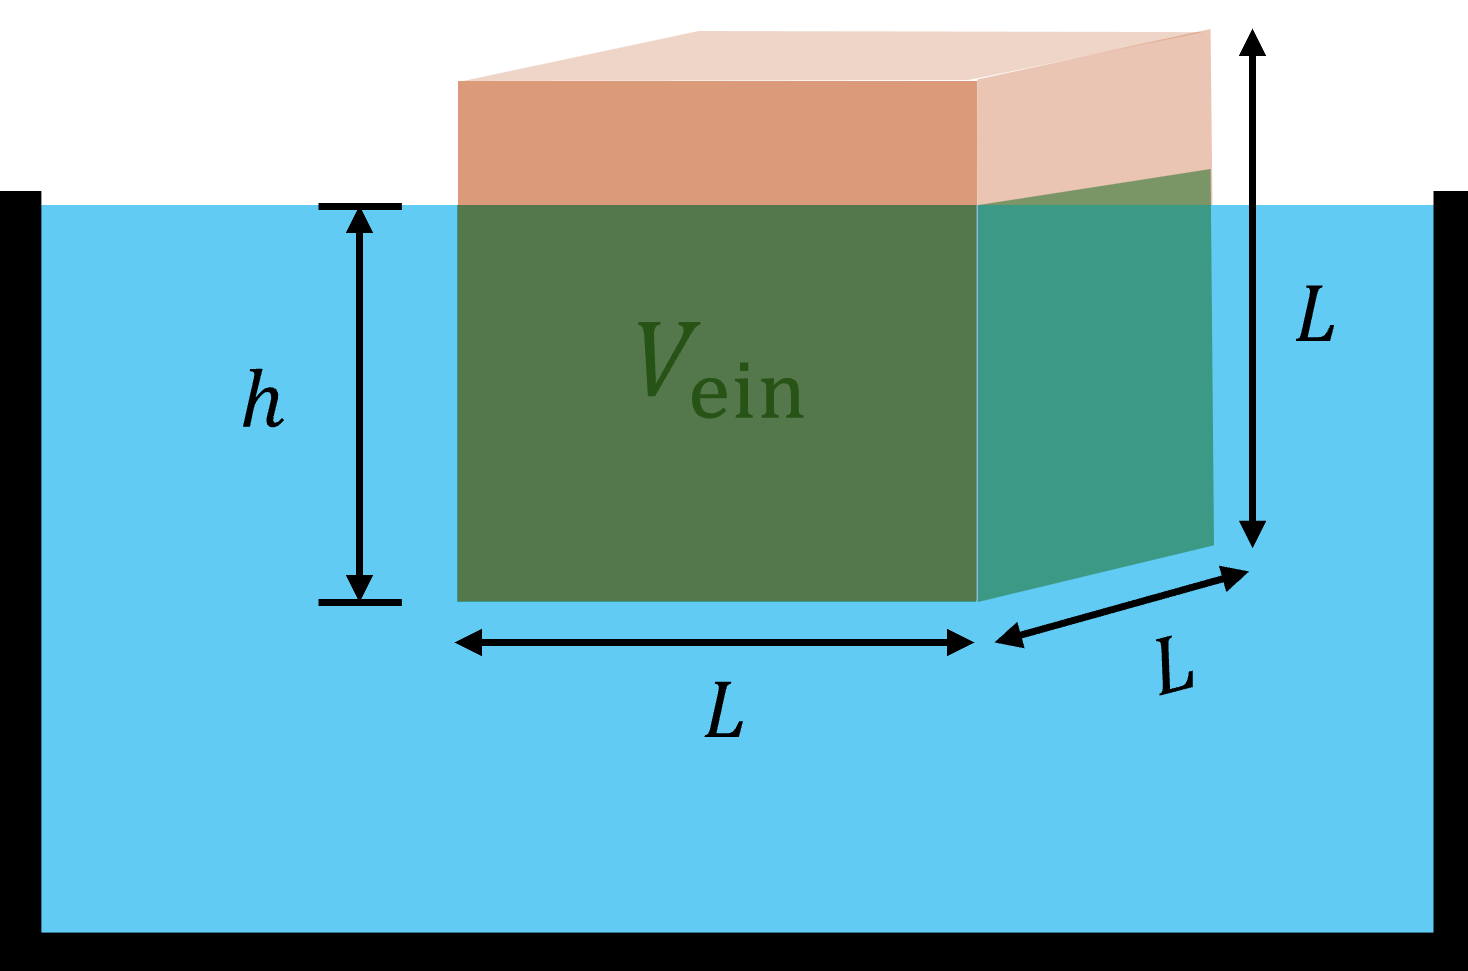
\includegraphics[width=0.4\textwidth]{Bilder/Test/3terAntritt/holzklotz_eintauchen.png}
\end{center}
Ein quaderförmiger Holzklotz mit einer Kantenlänge von $L = \SI{20}{\centi\metre}$ und einer Dichte von $\rho_{\text{Holz}} = \SI{750}{\kilogram\per\metre\cubed}$ wird in ein Wasserbecken gelegt. Die Dichte von Wasser beträgt $\rho_{\text{Wasser}} = \SI{1000}{\kilogram\per\metre\cubed}$. Der Auftrieb an der Luft kann vernachlässigt werden. Die Erdbeschleunigung ist $g = \SI{9.81}{\metre\per\second\squared}$.

\subsection*{Aufgabe}
Berechnen Sie eine Formel für die Eintauchtiefe $h$ des Holzklotzes. Wie tief taucht der Holzklotz in der Angabe in das Wasser ein?

\subsection*{Vorgehen}
\begin{enumerate}
    \item Formulieren Sie die Bedingung für das Schwimmen eines Körpers. Welche beiden Kräfte müssen sich im Gleichgewicht befinden?
    \item Berechnen Sie das Gesamtvolumen $V_{\text{ges}}$ des Holzklotzes und daraus seine Gewichtskraft $F_G$ (als Funktion der Kantenlänge $L$).
    \item Stellen Sie eine Formel für die Auftriebskraft $F_A$ auf. Diese soll vom Volumen des eingetauchten Teils des Klotzes ($V_{\text{ein}}$) abhängen.
    \item Das eingetauchte Volumen $V_{\text{ein}}$ kann durch die Grundfläche $A = L^2$ des Klotzes und die gesuchte Eintauchtiefe $h$ ausgedrückt werden. Setzen Sie dies in die Formel für die Auftriebskraft aus (3) ein.
    \item Setzen Sie die Formel für die Gewichtskraft aus (2) und die der Auftriebskraft aus (4) in (1) ein und lösen Sie die Gleichung nach der Eintauchtiefe $h$ auf.\\
    \textit{Lösung:} $h = L \cdot (\rho_{\text{Holz}}/\rho_{\text{Wasser}})$
    \item Wie tief taucht der Holzblock aus der Angabe ein?
\end{enumerate}

\vfill
\begin{flushright}
\renewcommand{\arraystretch}{1.23}
\begin{tabular}{|c | c | c | c | c | c|}
\hline
\multicolumn{6}{|l|}{\textbf{\large{Punkte: \quad\quad\quad /13}}}\\
\hline
% \textbf{1)} & \textbf{2)} & \textbf{3)} & \textbf{4)} & \textbf{5)} & \textbf{6)} \\
% \quad/1 & \quad/2 & \quad/2,5 & \quad/2,5 & \quad/3,5 & \quad/1,5 \\
% \hline
\end{tabular}
\end{flushright}

\newpage

\section*{Beispiel 4 - Single-Choice}
\textit{Kreuzen Sie die korrekte Antwort an. Pro Frage ist nur eine Antwort richtig.}

\begin{enumerate}[label=\arabic*.,itemsep=18pt]
    \item Welche physikalische Größe hat die SI-Einheit \si{\watt}?
    \begin{itemize}[label={$\square$},itemsep=1pt,topsep=0pt]
        \item Arbeit
        \item Energie
        \item Leistung
        \item Kraft
    \end{itemize}

    \item Bei einem isochoren Prozess eines idealen Gases bleibt welche Zustandsgröße konstant?
    \begin{itemize}[label={$\square$},itemsep=1pt,topsep=0pt]
        \item Der Druck
        \item Das Volumen
        \item Die Temperatur
        \item Die innere Energie
    \end{itemize}

    \item Verdoppelt sich die Geschwindigkeit eines Körpers, dann ändert sich seine kinetische Energie um welchen Faktor?
    \begin{itemize}[label={$\square$},itemsep=1pt,topsep=0pt]
        \item Faktor 2
        \item Faktor 4
        \item Faktor 6
        \item Faktor 8
    \end{itemize}

    \item Nach dem archimedischen Prinzip ist die Auftriebskraft gleich ...
    \begin{itemize}[label={$\square$},itemsep=1pt,topsep=0pt]
        \item dem Gewicht des Körpers.
        \item dem Gewicht des verdrängten Mediums.
        \item der Masse des Körpers geteilt durch sein Volumen.
        \item der Gewichtskraft der eingeschlossenen Luft.
    \end{itemize}

    \item Welche Aussage beschreibt das 3. Newtonsche Axiom?
    \begin{itemize}[label={$\square$},itemsep=1pt,topsep=0pt]
        \item Ohne resultierende Kraft bleibt die Geschwindigkeit konstant.
        \item Die Beschleunigung ist proportional zur Kraft.
        \item Kräfte treten paarweise als gleich große, entgegengesetzt gerichtete Wechselwirkungen auf.
        \item Energie kann nicht erzeugt oder vernichtet werden.
    \end{itemize}

    \newpage
    \item Ein Punkt auf dem Rand einer Scheibe hat den Abstand $r = \SI{0.5}{\metre}$ vom Mittelpunkt. Die Scheibe rotiert mit $\omega = \SI{6}{\radian\per\second}$. Wie groß ist die Bahngeschwindigkeit?
    \begin{itemize}[label={$\square$},itemsep=1pt,topsep=0pt]
        \item \SI{3}{\metre\per\second}
        \item \SI{6}{\metre\per\second}
        \item \SI{12}{\metre\per\second}
        \item \SI{0.083}{\metre\per\second}
    \end{itemize}

    \item Welche Aussage über Haft- und Gleitreibung ist im Allgemeinen richtig?
    \begin{itemize}[label={$\square$},itemsep=1pt,topsep=0pt]
        \item Die Gleitreibung ist stets größer als die maximale Haftreibung.
        \item Die maximale Haftreibung ist im Allgemeinen größer als die Gleitreibung.
        \item Beide sind immer gleich groß.
        \item Beide hängen nicht von der Normalkraft ab.
    \end{itemize}

    \item Die absolute Temperatur eines idealen Gases ist ein Maß für die ...
    \begin{itemize}[label={$\square$},itemsep=1pt,topsep=0pt]
        \item mittlere potentielle Energie der Teilchen.
        \item mittlere kinetische Energie der Teilchen.
        \item Anzahl der Teilchen.
        \item Dichte des Gases.
    \end{itemize}

    \item Der 1. Hauptsatz der Thermodynamik ist eine Formulierung des ...
    \begin{itemize}[label={$\square$},itemsep=1pt,topsep=0pt]
        \item Impulserhaltungssatzes.
        \item Energieerhaltungssatzes.
        \item Massenerhaltungssatzes.
        \item Gravitationsgesetzes.
    \end{itemize}

    \item Ein dünner Metallstab habe einen linearen Ausdehnungskoeffizienten von $\alpha = \SI{12e-6}{\per\kelvin}$. Wie lang ist der Stab bei einer Temperaturerhöhung von $\Delta T = \SI{50}{\kelvin}$, wenn seine ursprüngliche Länge $L_0 = \SI{2}{\metre}$ beträgt?
    \begin{itemize}[label={$\square$},itemsep=1pt,topsep=0pt]
        \item \SI{201.0012}{\metre}
        \item \SI{21.0012}{\metre}
        \item \SI{2.0012}{\metre}
        \item \SI{2.012}{\metre}
        \item \SI{2.120}{\metre}
        \item \SI{2.00012}{\metre}
        \item \SI{2.000012}{\metre}
    \end{itemize}
\end{enumerate}

\vfill
\begin{flushright}
\renewcommand{\arraystretch}{1.23}
\begin{tabular}{|l c|}
\hline
\multicolumn{2}{|l|}{\textbf{\large{Punkte: \quad\quad\quad /10}}}\\
\hline
\end{tabular}
\end{flushright}

\end{document}